%This is chapter 4
%%=========================================
\chapter[Results]{Results}
To test the validity of the implementation a series of slope stability simulations is run.
The results from these simulations is presented in the following sections.


\section{Homogenous isotropic soil - Zero variance}

To check the base case of spatialy invariant soil with known analytical solutions. This is to validate the input to the random field generation, the FEM mesh and calculation. The simulation is a elasto-plastic FEM simulation with Mohr-Columb material model using Plaxis undraind(C) behaviour. 15-Node triangular FEM elements are used. The slope is 5 meter high with a 2:1 gradient.
The soil parameters is presented in Table \ref{tab1}. The resulting random field, or in this particular case a constant field, is shown in Figure \ref{fig:p1} and the 2:1 slope geometry and Plaxis 2D mesh is shown in Figure \ref{fig:p2}.


\begin{table}[h]
	\centering\small
	\caption{Soil parameters for Homognus isotropic soil}
	\label{tab1}
		\begin{tabular*}{\textwidth}{@{\extracolsep{\fill}}lccc}
			\toprule
			 Soil model  &\multicolumn{3}{c}{Mohr Columb - Undrained(C)}\\
  \cmidrule{2-4}
			Statistical Soil	& Mean		 	& Coefficient of Variation 		& Scale of fluctuation \\
			Parameters	  	& $\mu$ 		&  $CoV = \frac{\sigma}{\mu}$ 		& $\theta$ \\
        
			\midrule
			  Unit weight, $\gamma_{sat}=\gamma{unsat}$ & 20 $kN/m^3$ & 0 & - \\
		          Modulus of elasticity, $E$ & 10 $MPa$ & 0 & - \\
		          Poissons ratio, $\nu$ & 0.49 & 0 & - \\
		          Undrained Shear Strength,$S_u$ & 20 $kPa$ & 0 & - \\
			\bottomrule
		\end{tabular*}
\end{table}

Running a Plaxis c-reduction calculation phase, plot in \ref{fig:psf1}, on the uniform soil slope gives a Factor of Safety, $F_s = 1.14$. The corresponding $F_s$ optaind by slope stability charts after \citet{Janbu1968slope} is $F_s = 1.16$. 

\begin{figure}[h]
	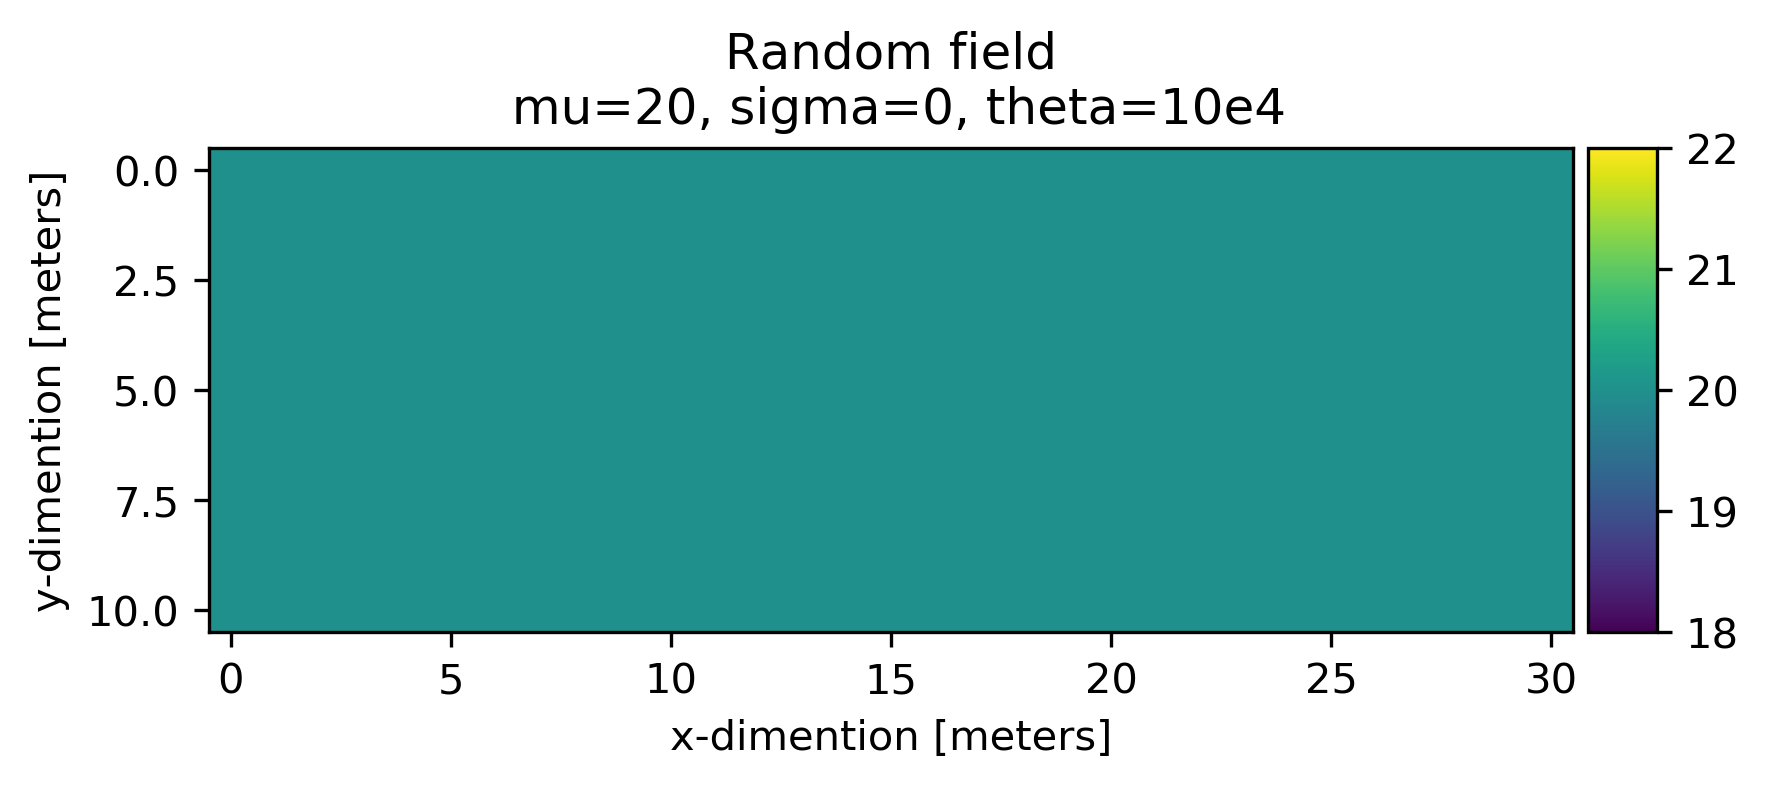
\includegraphics[width=\textwidth]{fig/testRF}
	\caption{$S_u$ Random field, in this particular case the soil strength is uniform}
	\label{fig:p1}
\end{figure}

\begin{figure}[h]
	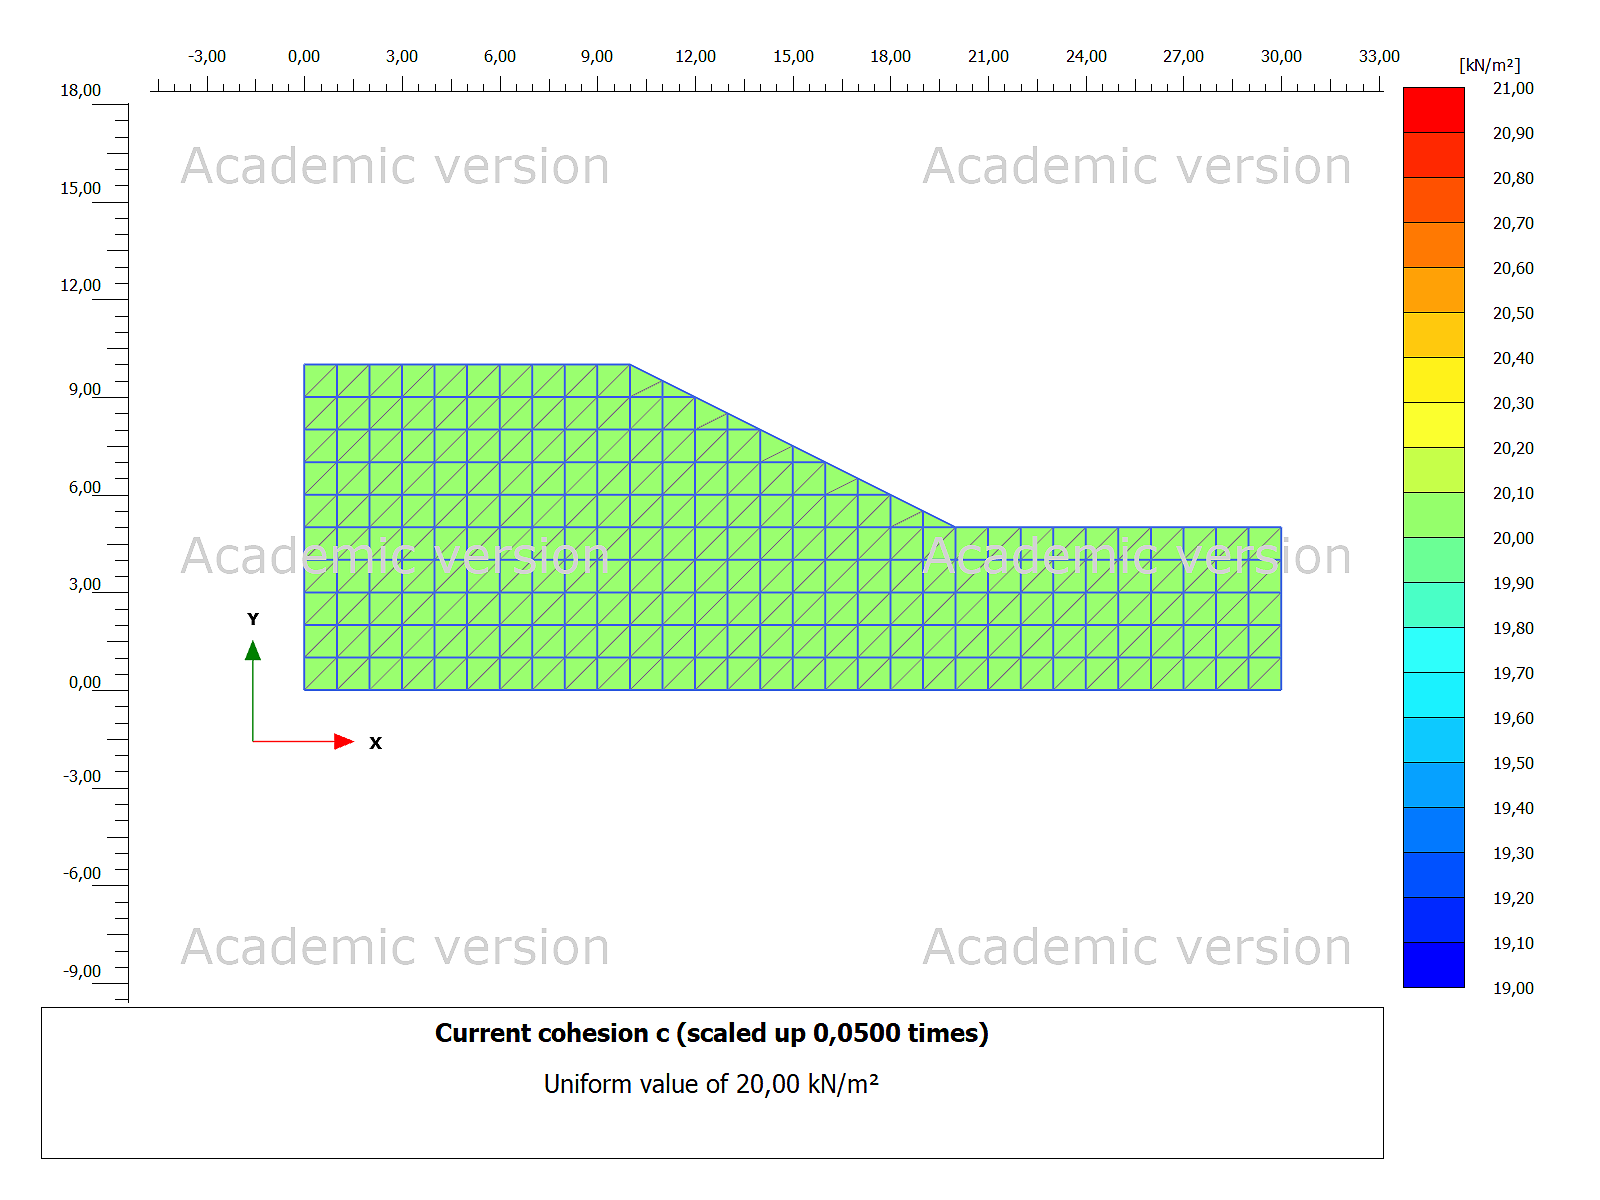
\includegraphics[width=\textwidth]{fig/testp}
	\caption{Slope geometry, with soil strength property from the random field maped to the soil Plaxis soil elements and triangular FEM elements displayed}
	\label{fig:p2}
\end{figure}

\begin{figure}[h]
	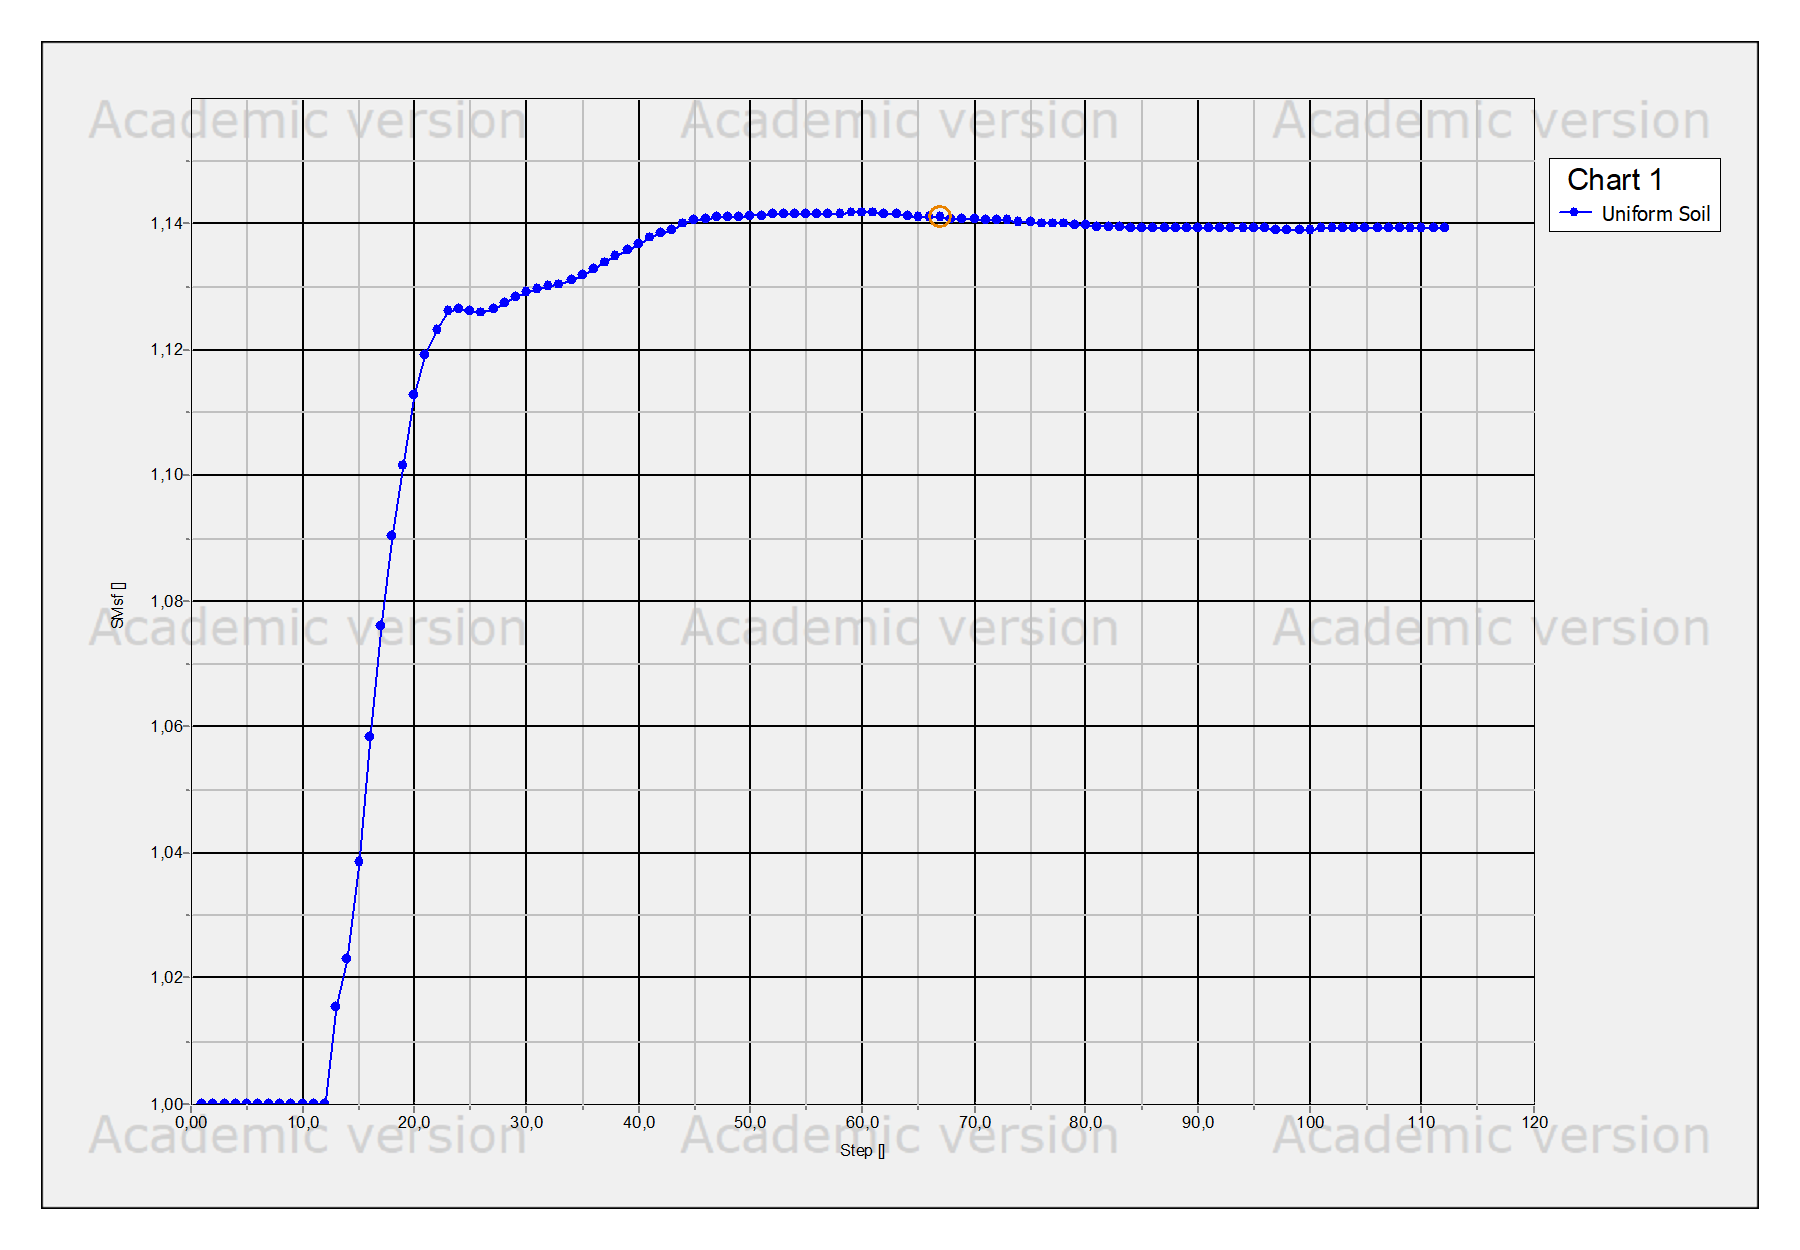
\includegraphics[width=\textwidth]{fig/Chart1}
	\caption{Plaxis Safety factor}
	\label{fig:psf1}
\end{figure}



\section{Homogenus anisotropic soil - Spatial correlation length 50 and 10, COV=0.3}

\begin{figure}[h]
	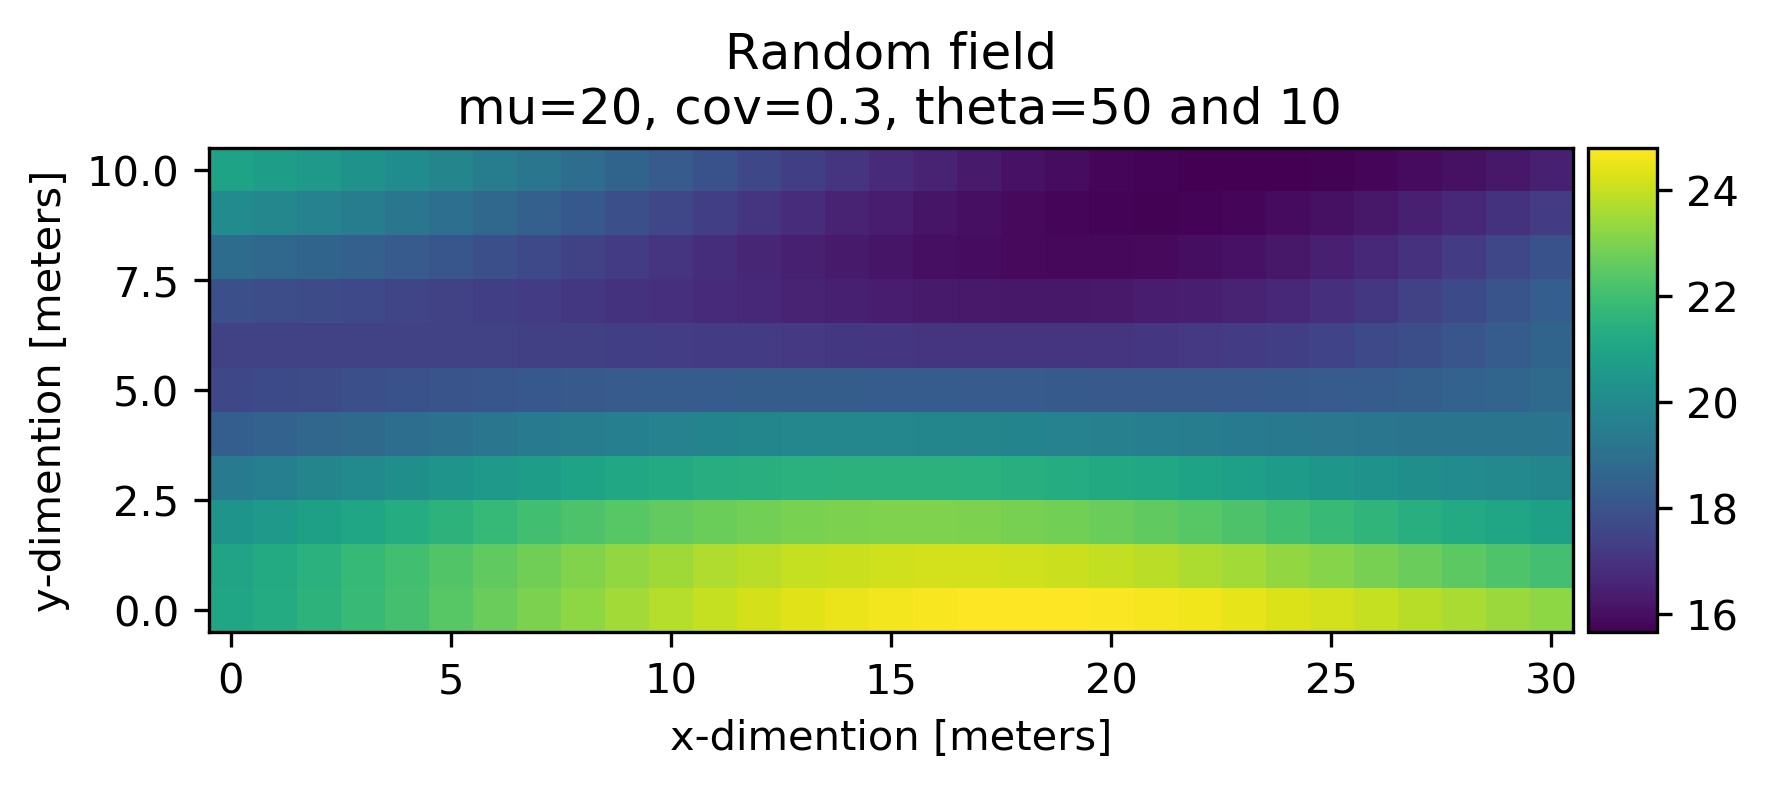
\includegraphics[width=\textwidth]{fig/testRF2}
	\caption{Random field}
	\label{fig:p3}
\end{figure}

\begin{figure}[h]
	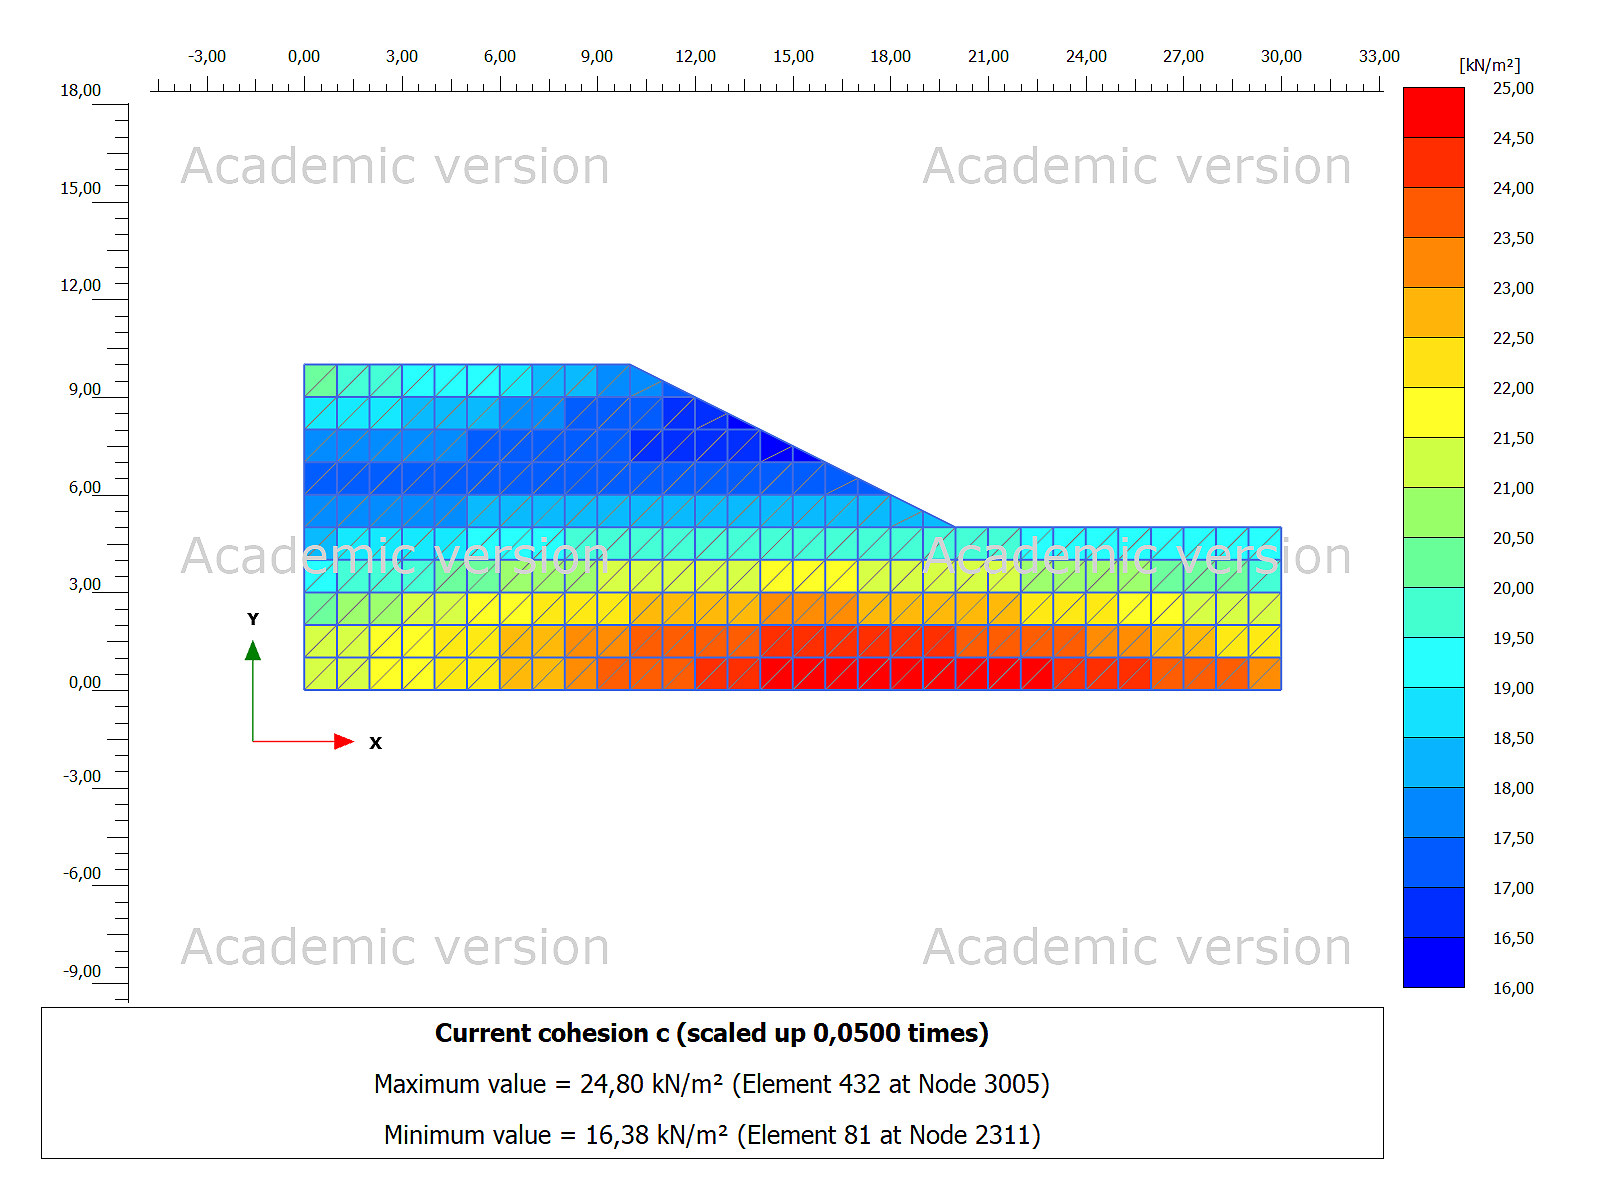
\includegraphics[width=\textwidth]{fig/testp2}
	\caption{Slope geometry}
	\label{fig:p4}
\end{figure}

